\iffalse
\silentchapter{Anexe}
%% Nu se pot face referinte pe silentchapter => nu are sens sa pun label
% \label{cap:anexe}

Anexe prezintă doar elementele specifice proiectului!

Anexele (dacă este cazul) constituie o secțiune separată a lucrării care nu se numerotează ca și capitol. Anexele se numerotează crescător cu numere arabe (ex.: Anexa 1, Anexa 2 etc.). Anexele vor conține scheme, diagrame, secvențe din codul sursă.

\section{Componente Software}
\label{anexa1:comp_soft}

% \textit{Componente software:}
\begin{itemize}
    \item diagramele UML care referă numai la componentele dezvoltate de student și care datorită complexității pot fi listate pe o foaie de tip A3 sau A2.
    \item cod sursă numai pentru componentele dezvoltate de către student.
\end{itemize}

%% inserati \newpage inaintea fiecarui \section cu anexa pentru ca fiecare anexa sa inceapa pe pagina noua
\newpage
\section{Componente Hardware}
\label{anexa2:comp_hard}

% \textit{Componente Hardware:}
\begin{itemize}
    \item schemele electrice finale realizate într-un CAD de profil; 
    \item schemele cablajelor realizate pentru implementare, realizate într-un CAD de profil;
    \item informații suplimentare despre implementarea și testarea aplicației (de ex. capturi de osciloscop);
    \item schemele standard ce vor fi folosite pentru testare (pseudocod sau schemă logică);
    \item extrase din foi de catalog. 
\end{itemize}

%% inserati \newpage inaintea fiecarui \section cu anexa pentru ca fiecare anexa sa inceapa pe pagina noua
\newpage
\section{Codul funcției xyz()}
\label{anexa3:func_xyz}

În Figura \ref{fig:AT} este prezentat unul dintre cele mai impunătoare vechicule ale Imperiului.

\begin{figure}[H]
    \centering
    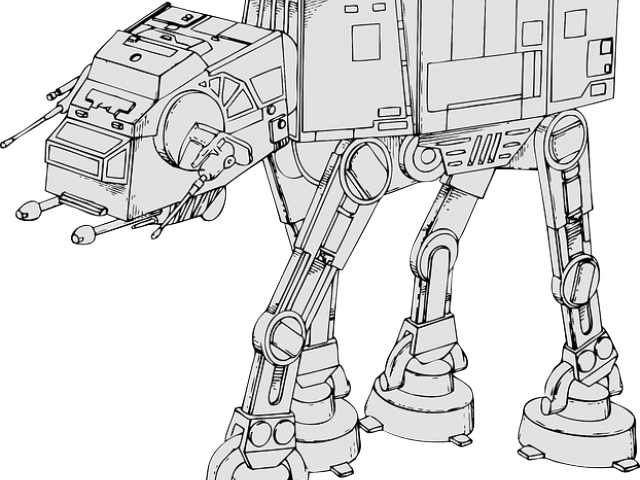
\includegraphics[width=0.5\textwidth]{anexe/figuri/AT.png}
    \caption{AT\protect\footnotemark}
    \label{fig:AT}
\end{figure}
\footnotetext{imagine preluată de pe un site web care nu „merită” trecut la bibliografie \url{https://www.pngitem.com/}}

\textcolor{gray}{\lipsum} (Figura \ref{fig:millennium_falcon})

\begin{figure}[H]
    \centering
    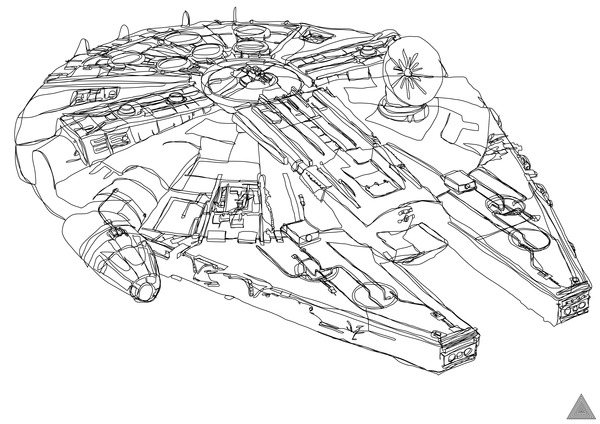
\includegraphics[width=0.8\textwidth]{anexe/figuri/millennium_falcon.jpeg}
    \caption{Millennium Falcon\protect\footnotemark}
    \label{fig:millennium_falcon}
\end{figure}
\footnotetext{imagine preluată de pe un site web care nu „merită” trecut la bibliografie \url{http://clipart-library.com/}}

%% inserati \newpage inaintea fiecarui \section cu anexa pentru ca fiecare anexa sa inceapa pe pagina noua
\newpage
\section{Tabel lung pe mai multe pagini}
\label{anexa4:long_table}

Malware (software rău intenționat) este un termen folosit pentru a descrie orice program sau cod care ocolește procesele de control al accesului, este creat cu intenția de a ataca un sistem de calcul sau rețea, pentru a provoca daune sau a compromite acel sistem. În categoria malware se includ: viruși, \textit{ransomware}, \textit{keyloggers}, troieni, viermi, \textit{spyware} etc (Tabelul \ref{tab_tipuri_de_malware}). În vocabularul curent, termenul de "virus" este folosit abuziv pentru orice tip de malware.

\begin{longtable}[c]{|l|p{6cm}|p{2cm}|}
	\caption{Tipuri de malware\label{tab_tipuri_de_malware}}\\
	
	\hline
	\multicolumn{1}{|c|}{\textbf{\textit{Tip}}} & 
	\multicolumn{1}{c}{\textbf{\textit{Descriere}}} & 
	\multicolumn{1}{|c|}{\textbf{\textit{Exemple elocvente}}}  \\
	\hline
	\endfirsthead
	
	\multicolumn{3}{c}{Continuarea tabelului \ref{tab_tipuri_de_malware}}\\
	\hline
	\multicolumn{1}{|c|}{\textbf{\textit{Tip}}} & 
	\multicolumn{1}{c}{\textbf{\textit{Descriere}}} & 
	\multicolumn{1}{|c|}{\textbf{\textit{Exemple elocvente}}}  \\
	\hline
	\endhead
	
	\hline
	\endfoot
	
	\hline
	\endlastfoot
	
	\multirow{8}*{Virus} &
	cod executabil malițios, atașat la fișiere sau programe legitime. Majoritatea virușilor necesită declanșarea de către utilizatorul final. Se răspândește prin intermediul unităților USB, discurilor optice, partajărilor în rețea sau e-mail-ului &
	%\multirow{6}*{Brain, Michelangelo, Melissa} \\  
	\newline \newline Brain, \newline Michelangelo, \newline Melissa \\
	\hline

	\multirow{5}{*}{Ransomware} & 
	conceput pentru a ține captiv un sistem informatic, de obicei prin criptarea datelor esențiale, dezactivează accesul victimei la date până la efectuarea unei plăți către atacator & 
	%\multirow{5}{*}{WannaCry, Petya} \\ 
	\newline WannaCry, \newline Petya \\	
	\hline
	
	\multirow{2}{*}{Fileless Malware} & 
	face modificări la fișierele native ale sistemului de operare & 
	\multirow{2}{*}{Astaroth} \\ 
	\hline
	
	\multirow{4}{*}{Spyware} & 
	proiectat pentru a urmări acțiunile utilizatorului și a colecta date despre activitatea victimei, fără cunoștința acesteia & 
	\multirow{4}{*}{DarkHotel} \\ 
	\hline
	
	\multirow{3}{*}{Adware} & 
	livrează anunțuri în mod automat. Unele sunt însoțite de programe \textit{spyware} & 
	\multirow{3}{*}{Fireball} \\ 
	\hline
	
	\multirow{5}{*}{Troian} & 
	execută operațiuni rău intenționate disimulate ca operațiuni dorite. Se deghizează în codul unui program cunoscut și se atașează de fișiere non-executabile & 
	\multirow{5}{*}{Emotet} \\ 
	\hline
	
	\multirow{7}{*}{Worms} & 
	se reproduce singur, se răspândește într-o rețea prin replicare, prin exploatarea vulnerabilităților din rețele. Au tipare similare, inclusiv o vulnerabilitate activă, o modalitate de a se propaga singuri și conțin un \textit{payload} & 
	\multirow{7}{*}{Stuxnet} \\ 
	\hline
	
	\multirow{9}{*}{Rootkit} & 
	conceput pentru a modifica sistemul de operare, astfel încât computerul să poată fi accesat de la distanță, printr-o portiță de acces. Rootkit-urile modifică privilegiile de acces, fișierele de sistem și instrumentele de monitorizare a sistemului, ceea ce le face foarte greu de detectat și eliminat & \multirow{9}{*}{Zacinlo} \\ 
	\hline
	
	\multirow{2}{*}{Keyloggers} & 
	monitorizează apăsările de taste ale victimei & 
	\multirow{2}{*}{Olympic Vision} \\ 
	\hline
	
	\multirow{3}{*}{Bots} & 
	lansează automat atacuri concertate si concentrate asupra sistemului țintă & 
	\multirow{3}{*}{Echobot} \\ 
	\hline
	
	\multirow{2}{*}{Mobile Malware} & 
	conțin cod specific (Android, iOS) infectării dispozitivele mobile & 
	\multirow{2}{*}{Triada} \\ 
	\hline	
\end{longtable}

%% inserati \newpage inaintea fiecarui \section cu anexa pentru ca fiecare anexa sa inceapa pe pagina noua
\newpage
\section{Tabel simplu}
\label{anexa5:simple_table}

Pentru a ușura lecturarea lucrării de diplomă recomandăm ca tabelele (dacă nu sunt prea mari) să nu fie împărțite (sparte) pe mai multe pagini.

\begin{table}[ht]
    \centering
    \caption{Rezultatele simulării}
    \begin{tabular}{|c|c|c|} 
        \hline
        \textbf{\textit{Tipul semnalului}} & \textbf{\textit{Durata}} & \textbf{\textit{Randamentul}} \\
        \hline
        sinusoidal & 10s & 99\% \\ 
        \hline
        dreptunghiular & 12s & 81\% \\
        \hline
        triunghiular & 15s & 89\% \\
        \hline
    \end{tabular}
    \label{tabel:2}
\end{table}

În Tabelul \ref{tabel:2} este prezentat un exemplu de formatare pentru un tabel cu cap de tabel orizontal.

%% inserati \newpage inaintea fiecarui \section cu anexa pentru ca fiecare anexa sa inceapa pe pagina noua
\newpage
\section{Cod în python}
\label{anexa6:listing_python}

\begin{code}
    \begin{minted}{python}
        import numpy as np
            
        def incmatrix(genl1,genl2):
            m = len(genl1)
            n = len(genl2)
            M = None #to become the incidence matrix
            VT = np.zeros((n*m,1), int)  #dummy variable
            
            #compute the bitwise xor matrix
            M1 = bitxormatrix(genl1)
            M2 = np.triu(bitxormatrix(genl2),1)
        
            for i in range(m-1):
                for j in range(i+1, m):
                    [r,c] = np.where(M2 == M1[i,j])
                    for k in range(len(r)):
                        VT[(i)*n + r[k]] = 1;
                        VT[(i)*n + c[k]] = 1;
                        VT[(j)*n + r[k]] = 1;
                        VT[(j)*n + c[k]] = 1;
                        
                        if M is None:
                            M = np.copy(VT)
                        else:
                            M = np.concatenate((M, VT), 1)
                        
                        VT = np.zeros((n*m,1), int)
            
            return M
    \end{minted} 
    \caption{Codul funcției \textit{incmatrix}} 
    \label{code:python_incmatrix}
\end{code}

%% inserati \newpage inaintea fiecarui \section cu anexa pentru ca fiecare anexa sa inceapa pe pagina noua
\newpage
\section{Cod în Kotlin (mai lung de o pagină)}
\label{anexa7:listing_kotlin}

\begin{code}
    \begin{minted}{kotlin}
internal inner class ScheduleAdapter : 
        RecyclerView.Adapter<CalendarSessionViewHolder>(),
        StickyHeaderHandler {
        
    private var schedule: MutableList<ScheduleItem> = mutableListOf()
    var data: List<SessionDataGroup> = emptyList()
        set(value) {
            updateSchedule(value)
            field = value
        }

    override fun onCreateViewHolder(
            parent: ViewGroup, 
            viewType: Int): CalendarSessionViewHolder {
        val view = when (viewType) {
            ScheduleItem.TYPE_SMALL ->
                    R.layout.item_schedule_session_header_small
            ScheduleItem.TYPE_LARGE -> 
                    R.layout.item_schedule_session_header_large
            else -> R.layout.item_schedule_session_card
        }

        val holder = layoutInflater.inflate(view, parent, false)
        return CalendarSessionViewHolder(holder, _favoriteNeedSync)
    }
    override fun getItemCount(): Int = schedule.size

    override fun onBindViewHolder(
        holder: CalendarSessionViewHolder, position: Int) {
        holder.show(schedule[position])
    }

    override fun getItemViewType(position: Int): Int {
        return schedule[position].type
    }
    private fun updateSchedule(groups: List<SessionDataGroup>) {
        val result = mutableListOf<ScheduleItem>()
        for (group in groups) {
            if (group.type == 0) {
                result += ScheduleItem.SmallHeader(
                    group.title, R.color.dark_grey_40
                )
                continue
            }
            if (group.type == 1) {
                result += ScheduleItem.LargeHeader(group)
                continue
            }

            result += ScheduleItem.LargeHeader(group)
            result += group.sessions.map { ScheduleItem.Card(it) }
        }

        schedule = result
    }
    override fun getAdapterData(): MutableList<*> = schedule
}
    \end{minted}
    \caption{clasa \textit{ScheduleAdapter}} 
    \label{code:kotlin_scheduleAdapter}
\end{code}

%% inserati \newpage inaintea fiecarui \section cu anexa pentru ca fiecare anexa sa inceapa pe pagina noua
\newpage
\section{Cod în XML (preluat din fisier)}
\label{anexa8:listing_xml}

\begin{code}
    \inputminted{xml}{anexe/coduri_sursa/pom.xml}
    \caption{Exemplu de cod XML preluat din fișier extern}
    \label{code:xml_pom}
\end{code}
\fi


\silentchapter{Anexe}
\section{Rezultate Statistice Generatoare}
\label{anexa1:rez_stat_gens}
\begin{figure}[H]
    \centering
    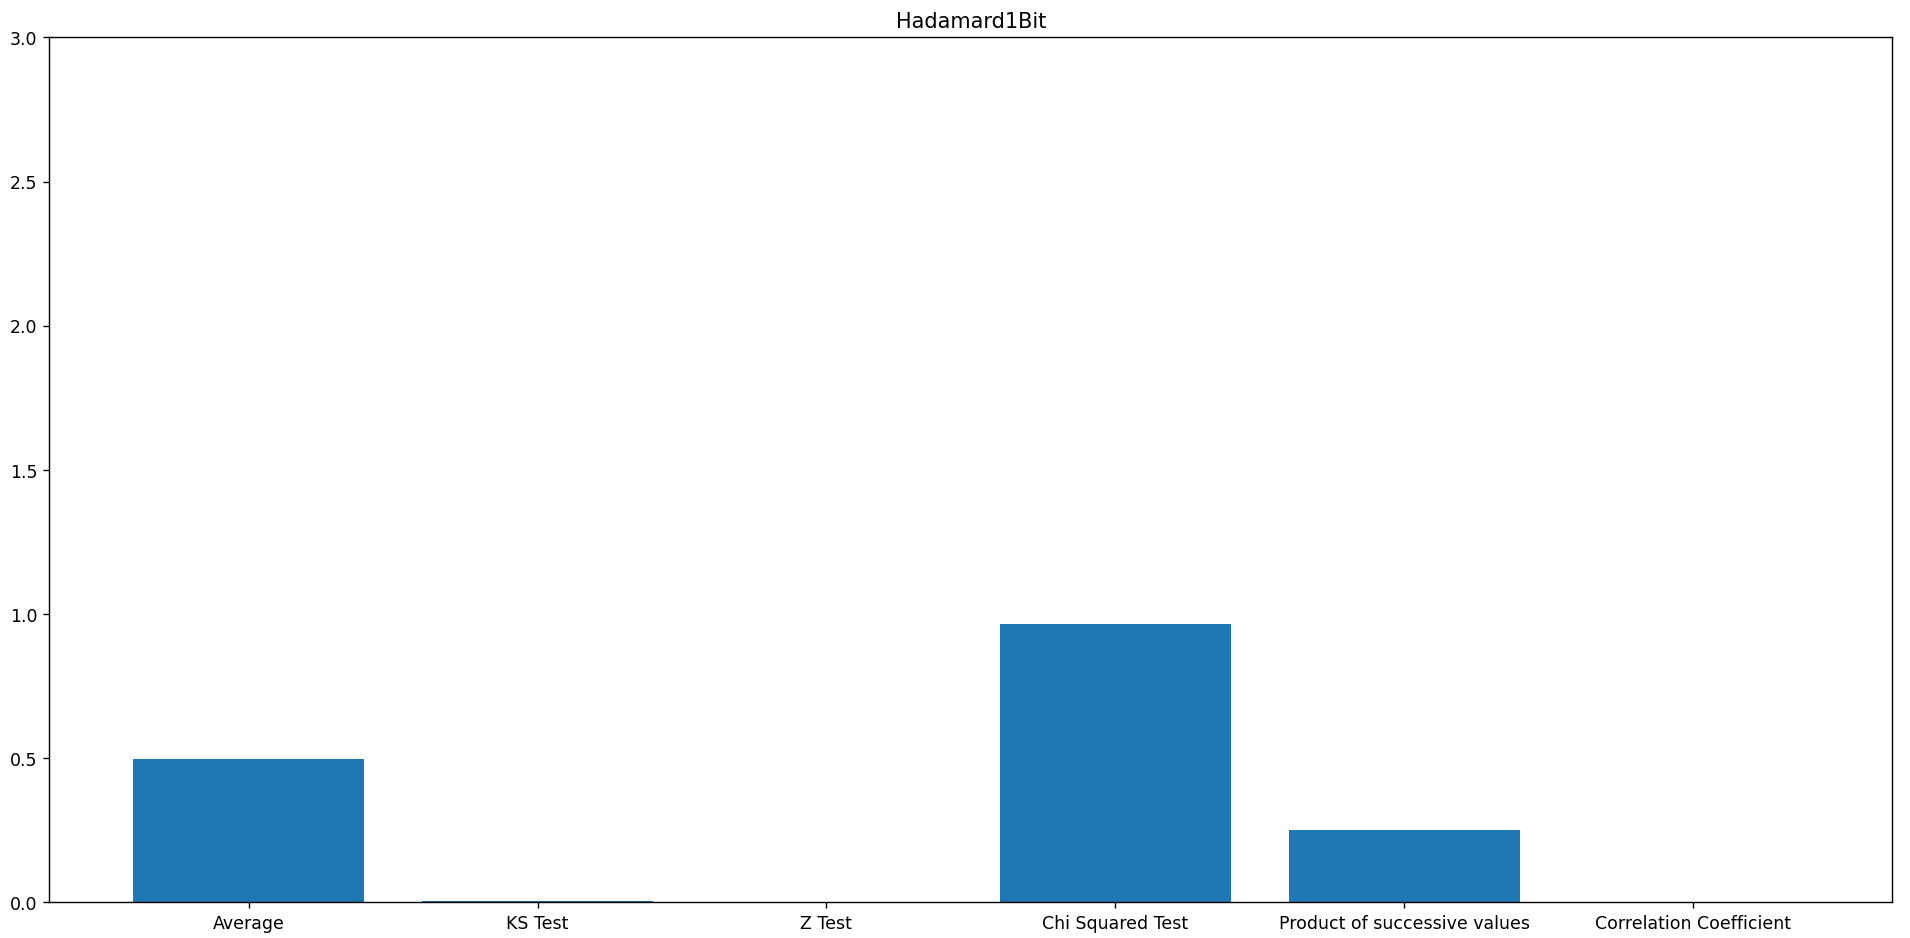
\includegraphics[width=1.0\textwidth]{continut/capitol4/figuri/StatsHadamard1Bit.png}
    \caption{Media statisticilor pentru un circuit cu o poartă Hadamard}
    \label{fig:StatsBarHadamard1Bit}
\end{figure}

\begin{figure}[H]
    \centering
    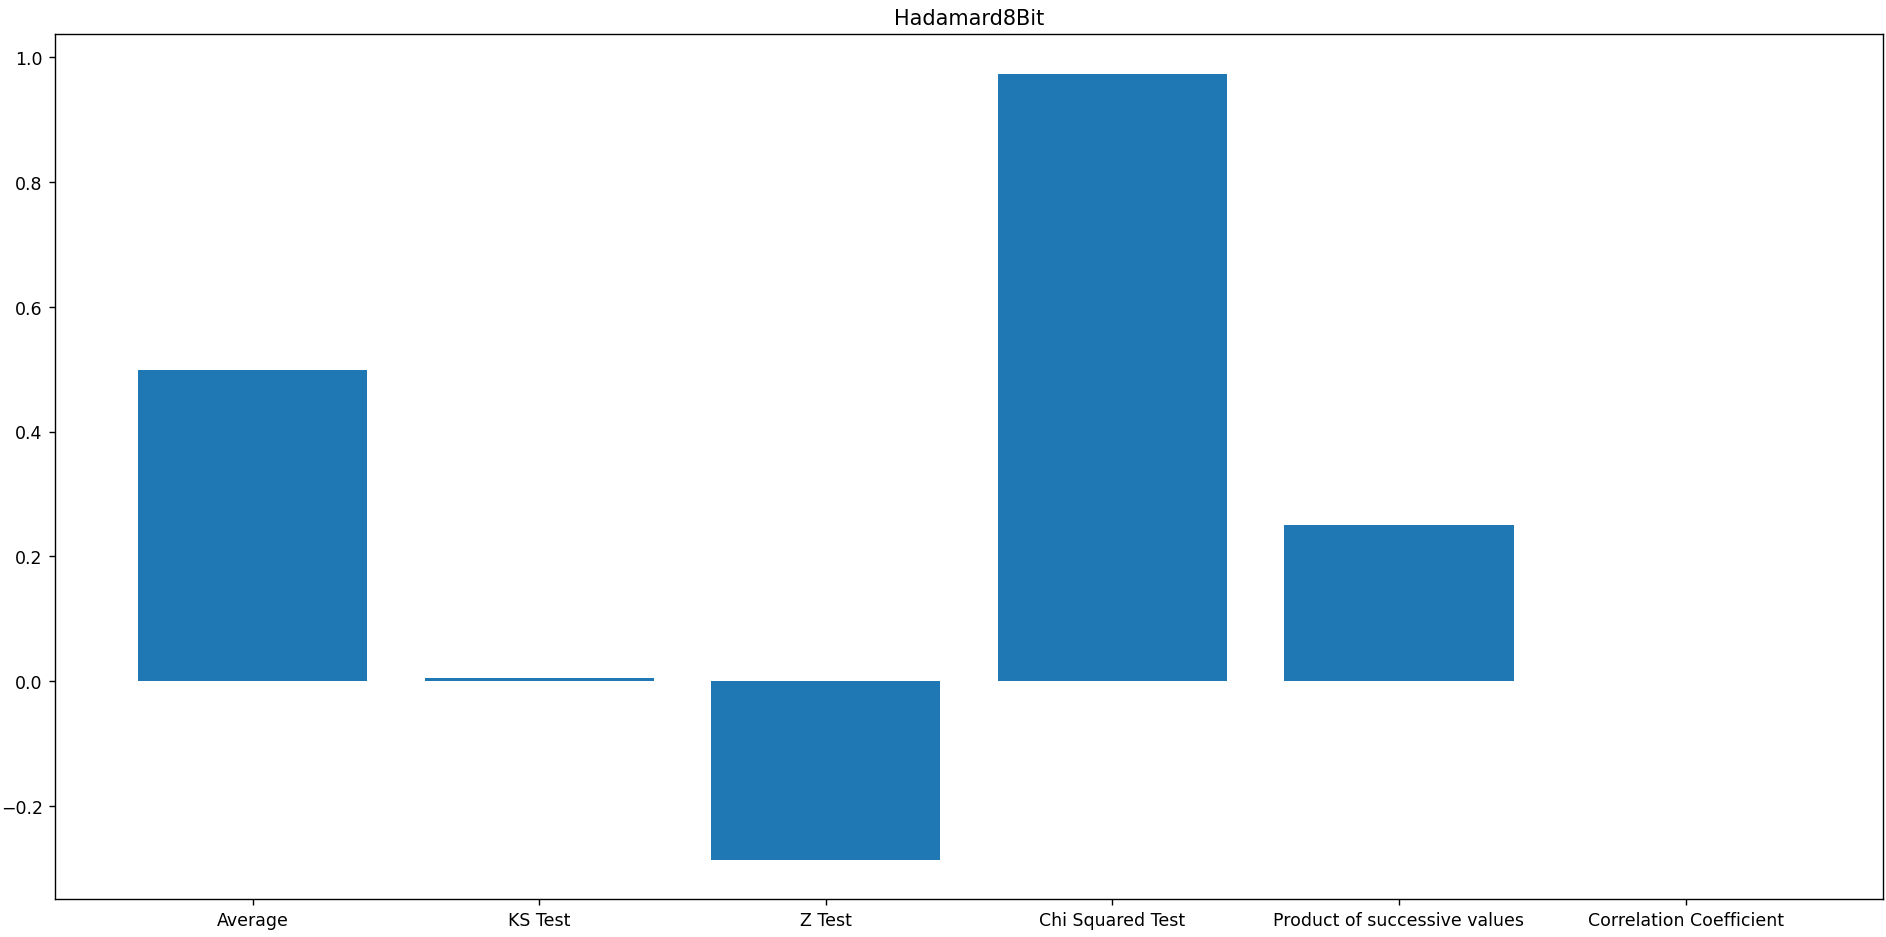
\includegraphics[width=1.0\textwidth]{continut/capitol4/figuri/StatsHadamard8Bit.png}
    \caption{Media statisticilor pentru un circuit cu 8 porți Hadamard}
    \label{fig:StatsBarHadamard8Bit}
\end{figure}

\begin{figure}[H]
    \centering
    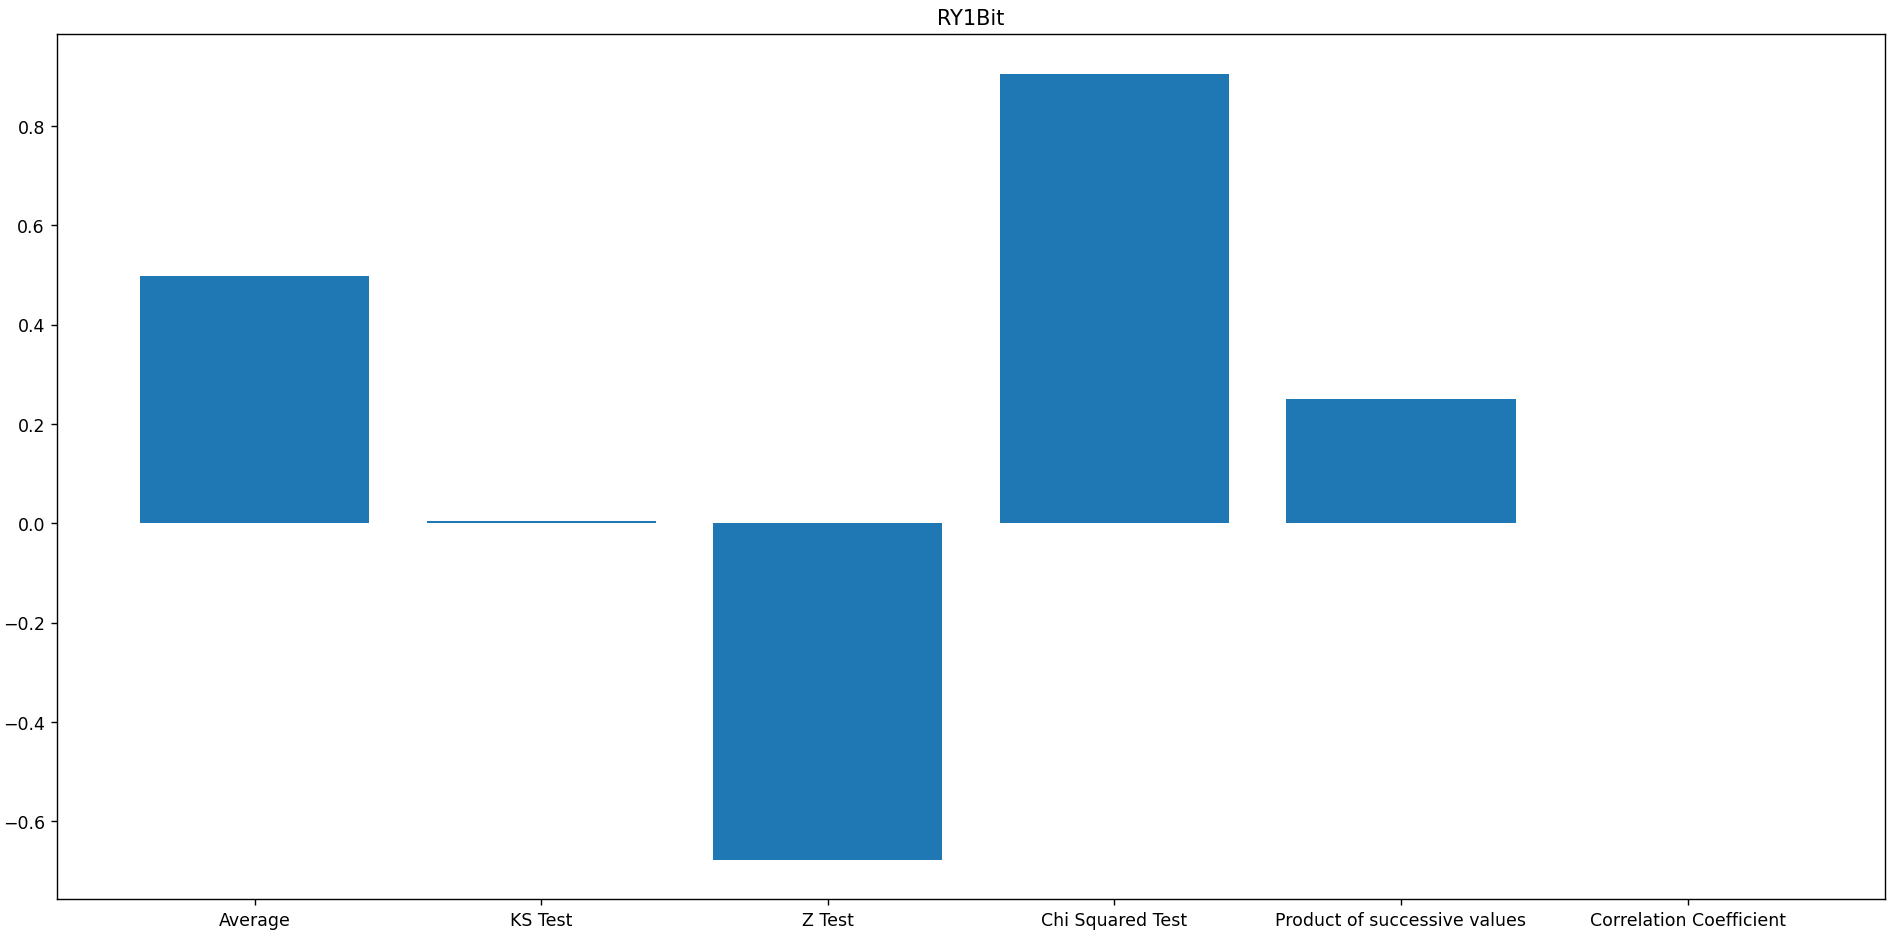
\includegraphics[width=1.0\textwidth]{continut/capitol4/figuri/StatsRY1Bit.png}
    \caption{Media statisticilor pentru un circuit cu o poartă RY($\pi/2$)}
    \label{fig:StatsBarRY1Bit}
\end{figure}

\begin{figure}[H]
    \centering
    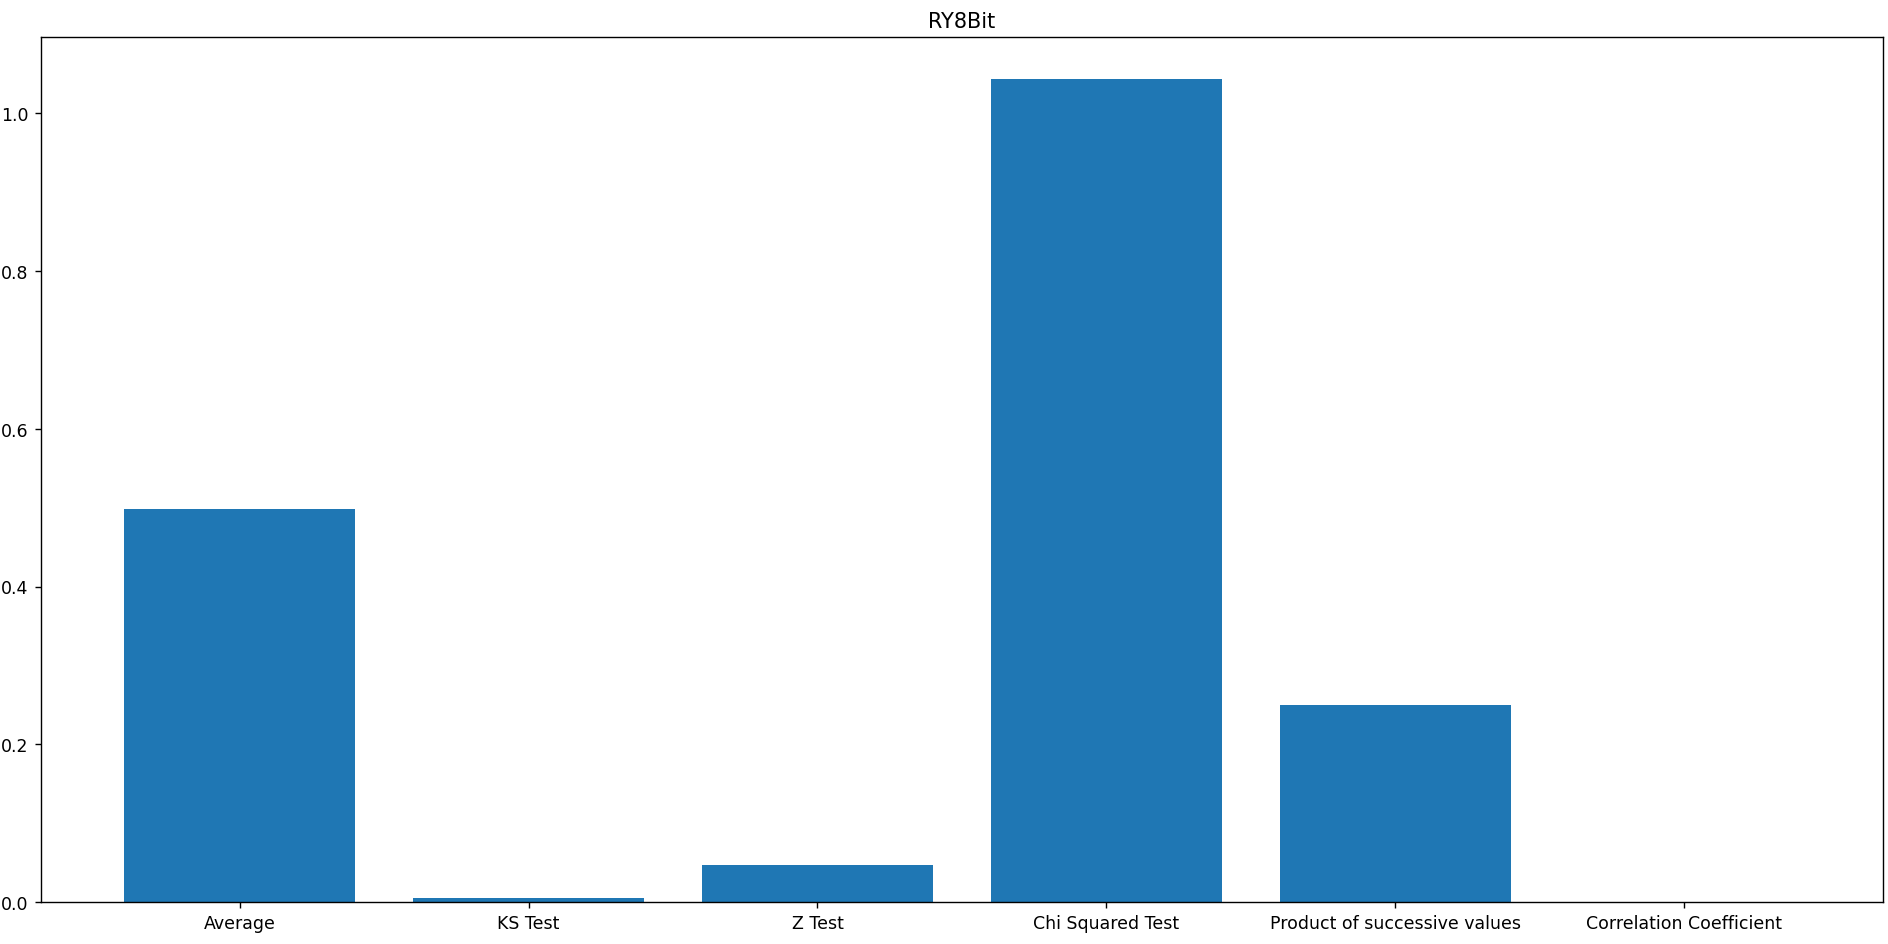
\includegraphics[width=1.0\textwidth]{continut/capitol4/figuri/StatsRY8Bit.png}
    \caption{Media statisticilor pentru un circuit cu 8 porți RY($\pi/2$)}
    \label{fig:StatsBarRY8Bit}
\end{figure}

\begin{figure}[H]
    \centering
    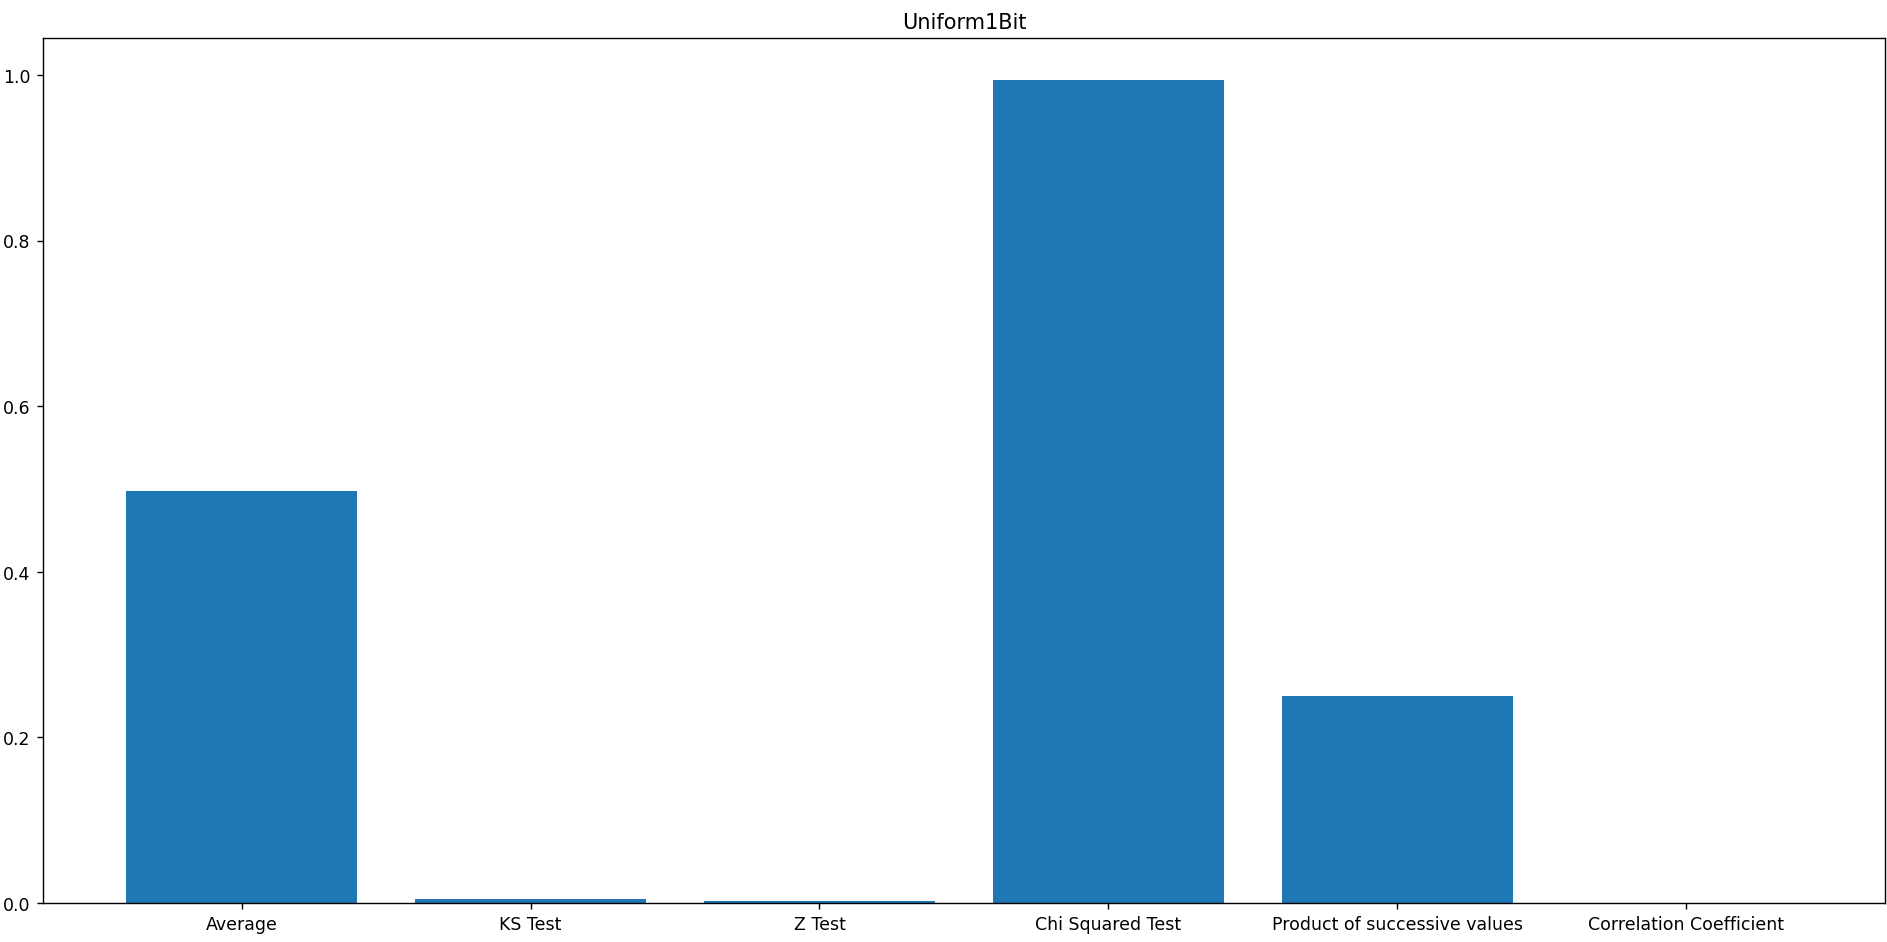
\includegraphics[width=1.0\textwidth]{continut/capitol4/figuri/StatsUniform1Bit.png}
    \caption{Media statisticilor pentru un circuit din biblioteca qiskit.finance cu 1 qubit}
    \label{fig:StatsBarUniform1Bit}
\end{figure}

\begin{figure}[H]
    \centering
    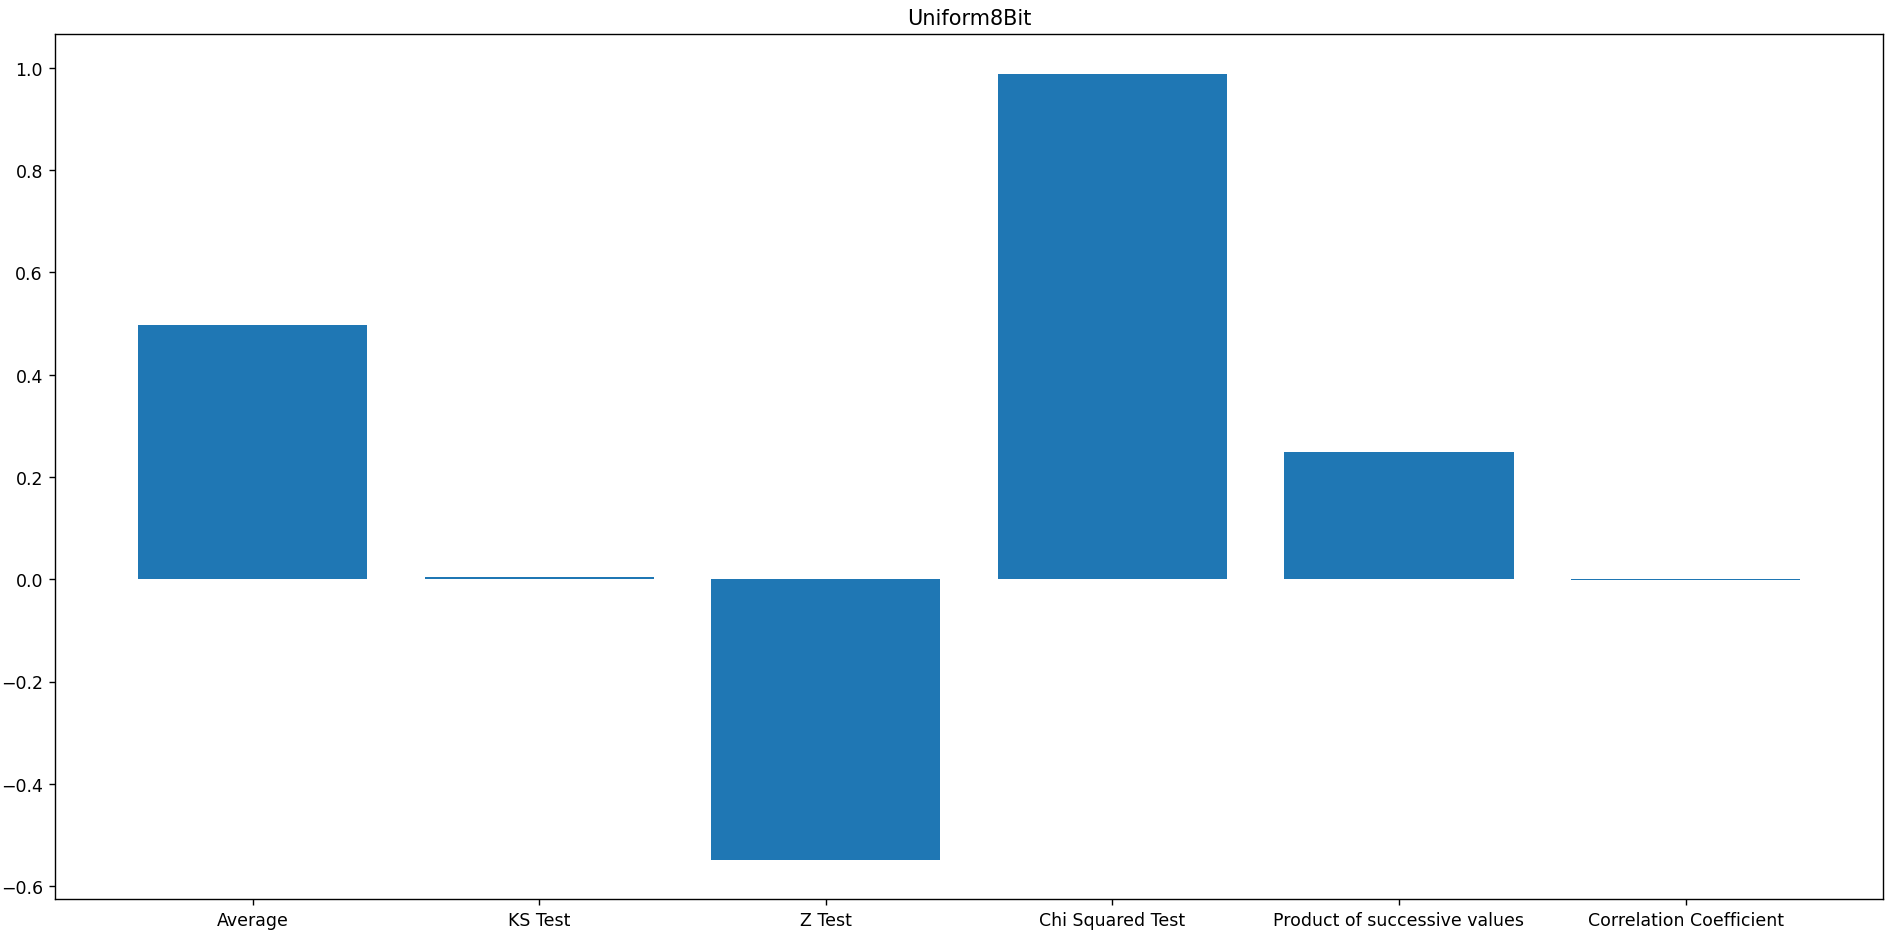
\includegraphics[width=1.0\textwidth]{continut/capitol4/figuri/StatsUniform8Bit.png}
    \caption{Media statisticilor pentru un circuit din biblioteca qiskit.finance cu 8 qubiți}
    \label{fig:StatsBarUniform8Bit}
\end{figure}

\begin{figure}[H]
    \centering
    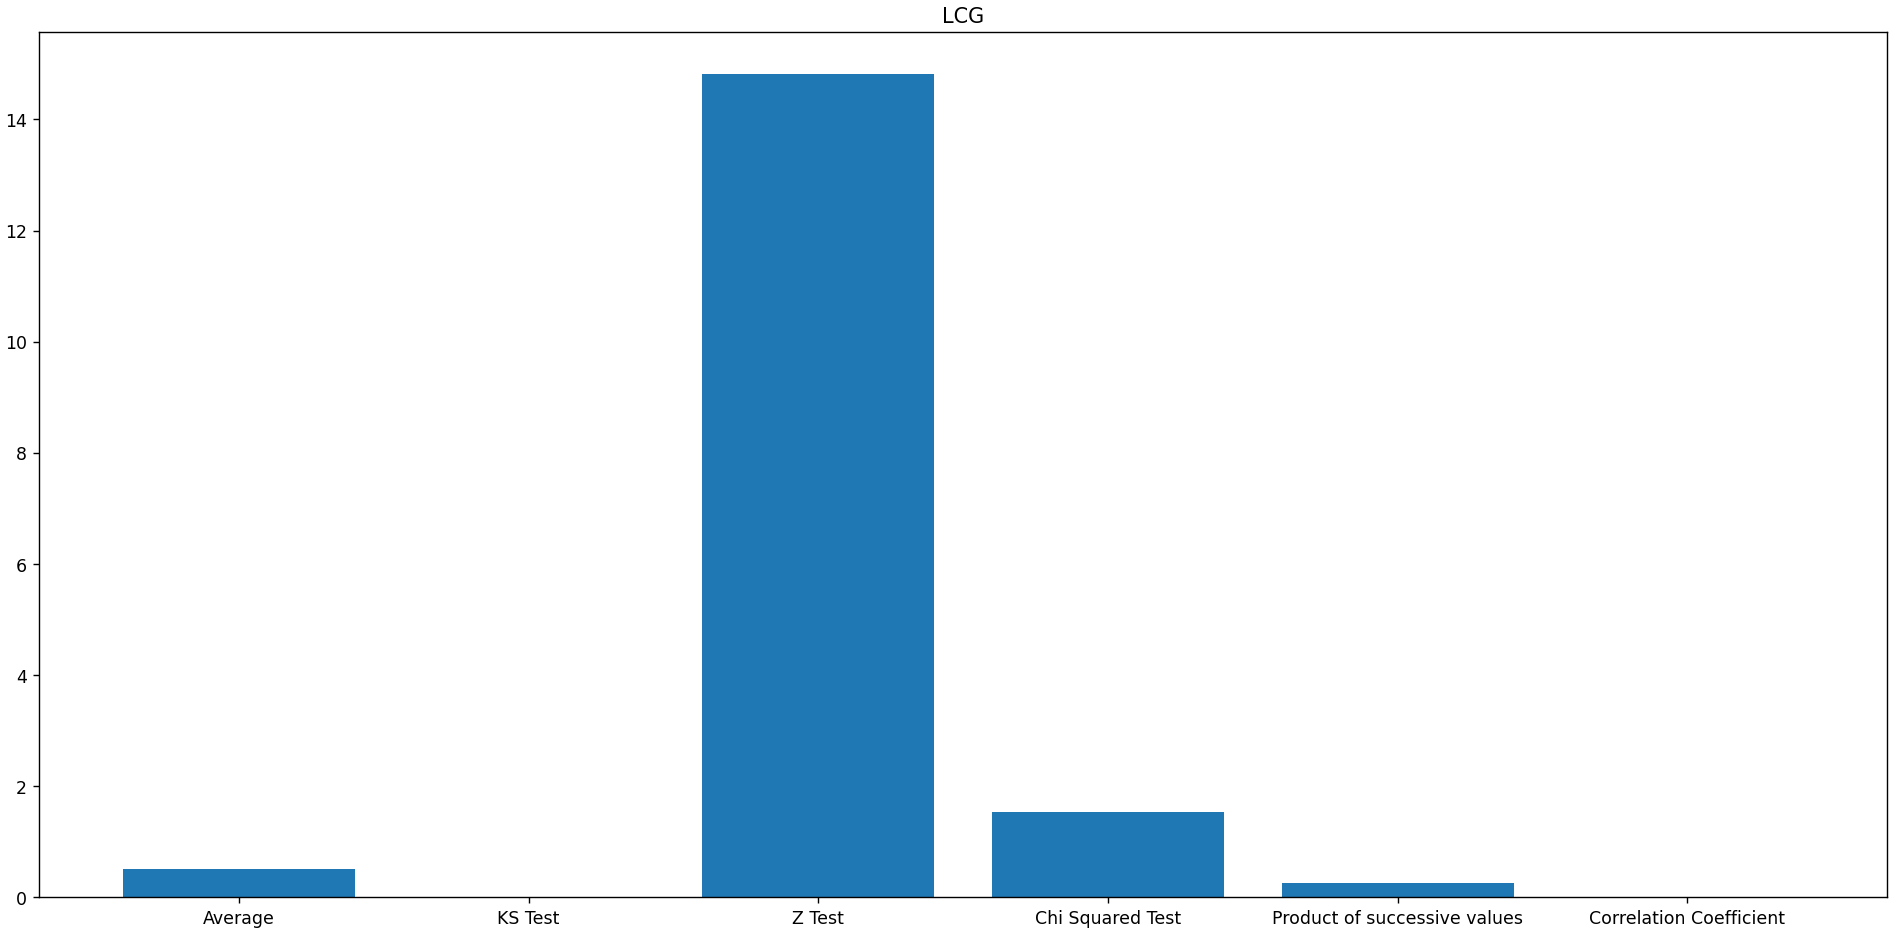
\includegraphics[width=1.0\textwidth]{continut/capitol4/figuri/StatsLCG.png}
    \caption{Media statisticilor pentru un PRNG cu algoritmul LCG}
    \label{fig:StatsBarLCG}
\end{figure}

\begin{figure}[H]
    \centering
    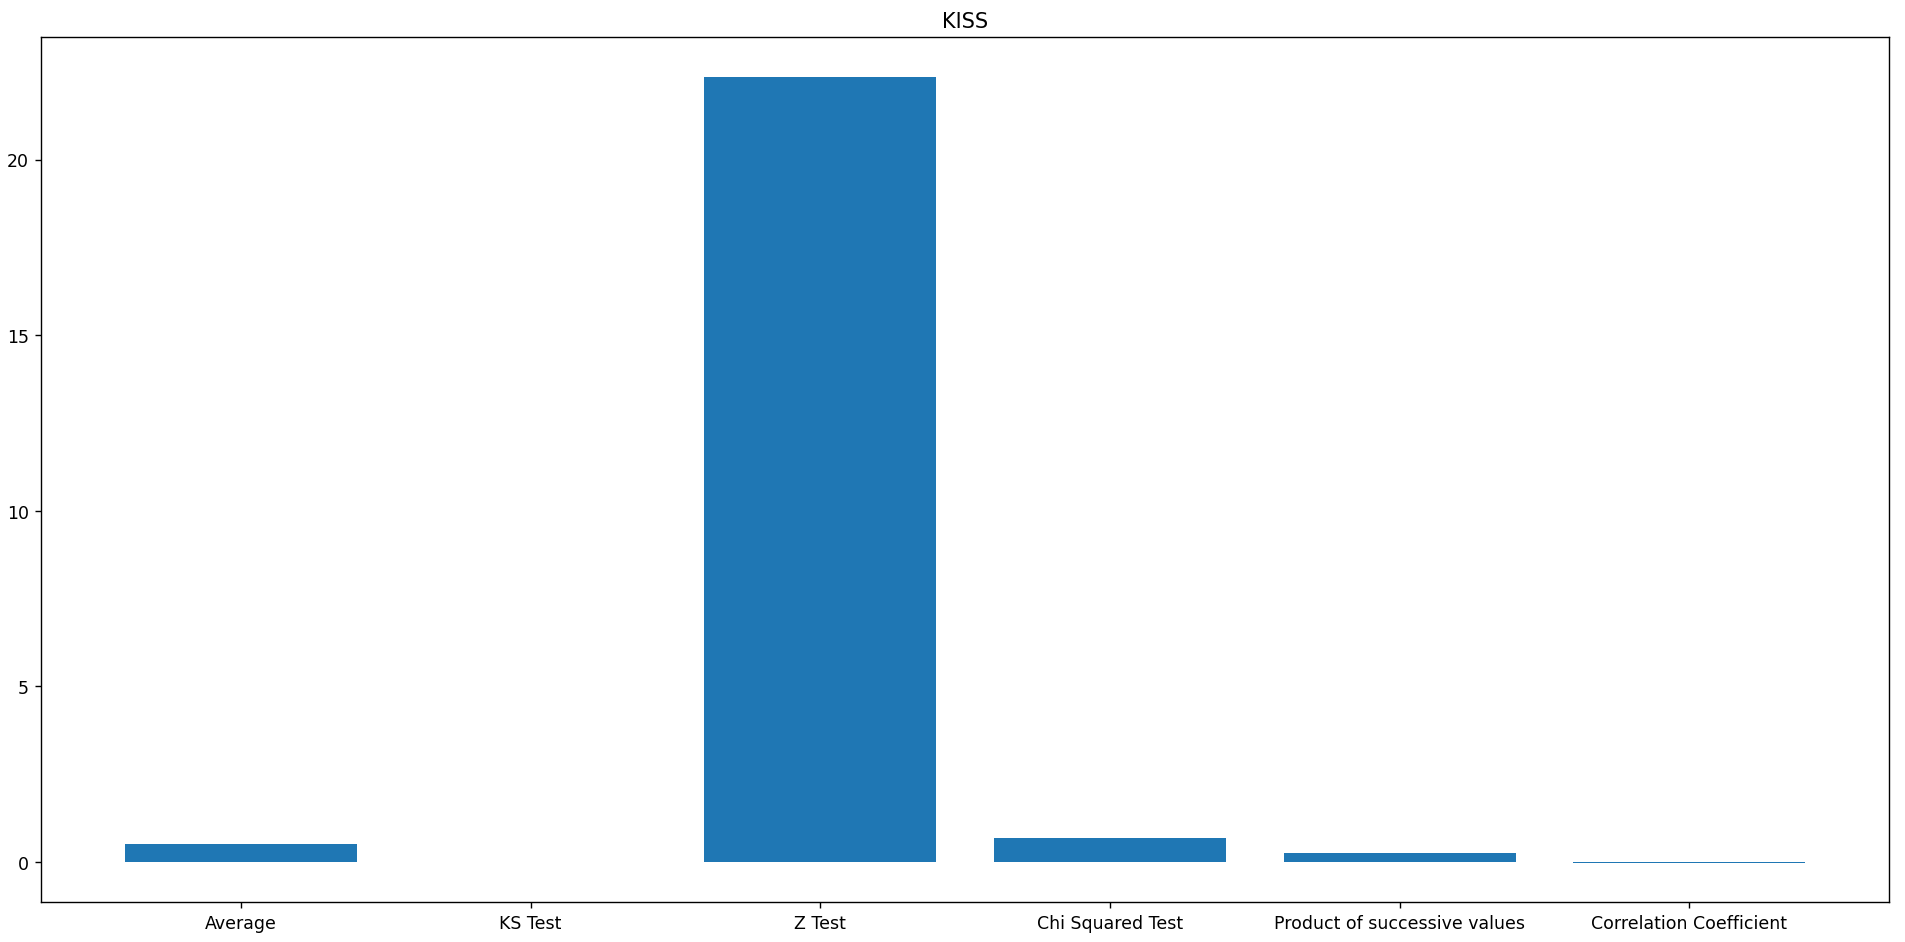
\includegraphics[width=1.0\textwidth]{continut/capitol4/figuri/StatsKISS.png}
    \caption{Media statisticilor pentru un PRNG cu algoritmul KISS}
    \label{fig:StatsBarKISS}
\end{figure}

\begin{figure}[H]
    \centering
    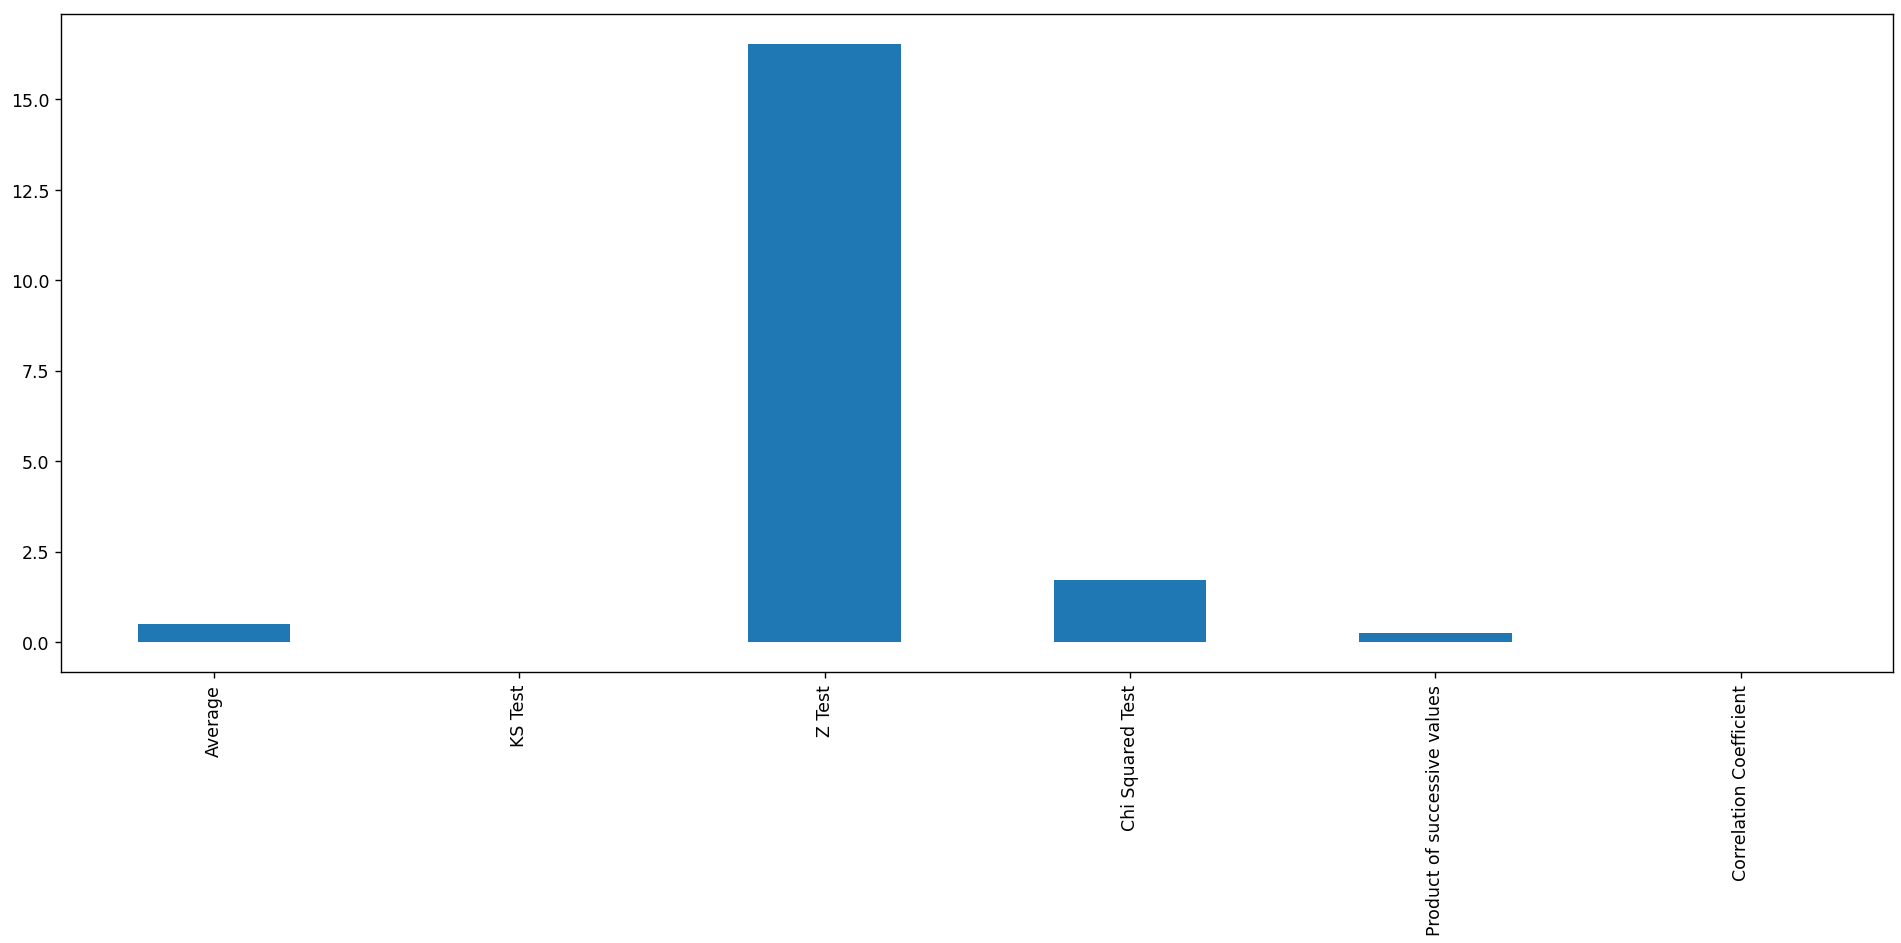
\includegraphics[width=1.0\textwidth]{continut/capitol4/figuri/StatsHWRNG.png}
    \caption{Media statisticilor pentru HWRNG}
    \label{fig:StatsBarHWRNG}
\end{figure}
\newpage

\section{Implementarea aplicației cu interfață utilizator}
\label{anexa2:GUIApp}
\begin{code}
\begin{minted}[linenos,tabsize=1,breaklines]{Python}
left_part = [
        [
            sg.Listbox(values=list(itertools.chain(*[[x for x in qrngs.QRNGs.keys()], [x for x in prngs.generators]])), key='-LISTBOX-', size=(30,None), expand_x=True, expand_y=True, enable_events=True)
        ]
    ]
    right_part = [
        [
             sg.Text('Simulated Mode', key='-MODE_TEXT-', text_color='green') 
        ],
        [
            sg.Canvas(key='-CANVAS-', size=(650,550))
        ],
        [
            sg.Text("Amount of numbers: "), sg.Input(key='-NUMS-', size=(30,1)), sg.Button('Generate', disabled=True, key='-GENERATE_BUTTON-'),
            sg.Button('Get Numbers', disabled=True, key='-NUMBERS_BUTTON-')
        ],
        [
            sg.Button('Run Box-Muller', disabled=True, key='-BOX-MULLER_BUTTON-'), sg.Button('See Circuit', disabled=True, key='-CIRCUIT_BUTTON-')
        ]
        
    ]

    menu_def = [['&Mode',  ['Simulated', 'Real']], ['&Help']]
    layout_main = [
        [sg.Menu(menu_def, tearoff=False, key='-MENU-', font=AppFont)],
        [sg.Column(left_part, expand_y=True), sg.VSeparator(), sg.Column(right_part, element_justification='center')]
    ]
    layout_statistics = [
        [sg.Multiline(size=(100,30), key='-STATISTICS_BOX-')]
    ]
    tabbed_layout = [[sg.TabGroup([[sg.Tab('MainTab', layout_main), sg.Tab('Statistics', layout_statistics)]])]]
\end{minted}
\caption{Definirea layout-urilor cu framework-ul PySimpleGUI}
\end{code}
\newpage
\begin{code}
\begin{minted}[linenos,tabsize=1,breaklines]{python}
if event == '-GENERATE_BUTTON-':
    _VARS['window']['-NUMBERS_BUTTON-'].update(disabled=False)
    if generator_string in qrngs.QRNGs.keys():
        prev_time = Timer()
        nums = qrngs.run_circuit(generator_string, int(values['-NUMS-']))
        time = Timer()
        if generator_string[0:6] != 'Normal':
            _VARS['window']['-BOX-MULLER_BUTTON-'].update(disabled=False)
        else:
            _VARS['window']['-BOX-MULLER_BUTTON-'].update(disabled=True)
        _VARS['window']['-CIRCUIT_BUTTON-'].update(disabled=False)
    else:
        prev_time = Timer()
        RNG = getattr(prngs, prngs.function_map[generator_string])
        time = Timer()
        nums = RNG(int(values['-NUMS-']))
        _VARS['window']['-BOX-MULLER_BUTTON-'].update(disabled=False)
        _VARS['window']['-CIRCUIT_BUTTON-'].update(disabled=True)
    _VARS['window']['-STATISTICS_BOX-'].update('')
    stats = generate_descriptive_stats(nums)
    for stat in stats:
        _VARS['window']['-STATISTICS_BOX-'].print(stat + ': ' + str(stats[stat]))
    _VARS['window']['-STATISTICS_BOX-'].print(f"Time to execute: {time - prev_time} seconds")
    if _VARS['plt_fig'] == False:
        draw_chart(nums)
    else:
        update_chart(nums)
    ran_box_muller = 0
\end{minted}
\caption{Implementarea funcționalității butonului de generare din aplicație}
\end{code}
\newpage
\begin{code}
\begin{minted}[breaklines, tabsize=1]{python}
if event == 'Real':
    _VARS['login_window'] = make_login_window()
    while True:
        event, values = _VARS['login_window'].read(timeout=500)
        if event == '-LOGIN_BUTTON-':
            API_KEY = values['-API_KEY-']
            _VARS['login_window'].Close()
            _VARS['window']['-MODE_TEXT-'].update(value='Real Mode', text_color='red')
            qrngs.API_KEY = API_KEY
            qrngs.login()
            sg.Popup(f'Real mode engaged! Quantum computer {qrngs.backend.name()} has only {qrngs.backend.configuration().n_qubits} Qubits! Not all Circuits implemented!', title='REAL MODE WARNING')
            break

if event == 'Simulated':
    API_KEY = None
    qrngs.API_KEY = None
    _VARS['window']['-MODE_TEXT-'].update(value='Simulated Mode', text_color='green')
\end{minted}
\caption{Implementarea determinării modului de acțiune (real sau simulat)}
\end{code}

\newpage

\section{Implementarea testelor statistice}
\label{anexa3:TesteStatistice}
\begin{code}
\begin{minted}[breaklines, tabsize=1]{python}
def KS_uniform(nums):
    nums = np.clip(np.divide(nums, 255), 0.0001, 0.9999)
    D_plus = 0
    D_minus = 0
    N = len(nums)
    memory_cdf = np.sort(nums)
    arange1 = np.arange(1.0, N + 1) / N
    arange2 = np.arange(0.0, N) / N
    D_plus = (arange1 - memory_cdf).max()
    D_minus = (memory_cdf - arange2).max()
    return(max(D_plus, D_minus))
\end{minted}
\caption{Implementarea testului Kologomorov-Smirnov}
\end{code}

\begin{code}
\begin{minted}[breaklines, tabsize=1]{python}
def prod_succ(nums):
    nums = np.array(nums)
    nums = nums / max(nums)
    sum = 0
    for i in range(1, len(nums)):
        sum += nums[i] * nums[i-1]
    coef = 1 / (len(nums) - 1) * sum
    return coef
\end{minted}
\caption{Implementarea testului produselor elementelor succesive, propus în \cite{art:PetrilaMantaUnguranu:IEEESystheory:2014}.}
\end{code}

\begin{code}
\begin{minted}[breaklines, tabsize=1]{python}
def correlation(nums):
    sum1 = 0
    sum2 = 0
    nums = np.array(nums)
    avg = np.average(nums)
    N = len(nums)
    for i in range(1, N):
        sum1 += (nums[i] - avg) * (nums[i-1] - avg)
    sus = N * sum1
    for i in range(N):
        sum2 += ( nums[i] - avg ) ** 2
    jos = (N - 1) * sum2
    coef = sus / jos
    return coef
\end{minted}
\caption{Implementarea formei coeficientului de corelație propus în \cite{art:PetrilaMantaUnguranu:IEEESystheory:2014}.}
\end{code}

\begin{code}
\begin{minted}[breaklines, tabsize=1]{python}
def generate_descriptive_stats(nums):
    dict_for_df = {
        'nums': nums
    }
    df = pd.DataFrame.from_dict(dict_for_df)
    stats = {}
    stats['min'] = df['nums'].min()
    stats['max'] = df['nums'].max()
    stats['count'] = len(df['nums'])
    stats['uniques'] = len(set(df['nums']))
    stats['25%'] = df['nums'].quantile(q=0.25)
    stats['50%'] = df['nums'].quantile(q=0.5)
    stats['75%'] = df['nums'].quantile(q=0.75)
    stats['mode'] = df['nums'].mode()[0]
    stats['std'] = df['nums'].std()
    stats['mean'] = df['nums'].mean()
    stats['median'] = df['nums'].median()
    stats['skew'] = df['nums'].skew()
    stats['kurtosis'] = df['nums'].kurt()
    stats['Kologomorov-Smirnov test vs. uniform (value should be very close to 0 for uniform):'] = KS_uniform(nums)
    stats['Z-test vs. uniform (Value should be <-2.5 or >2.5: '] = Z_test(nums)
    stats['Chi squared test for uniformity (Value should be close to 1 for uniform): '] = chi_2_test(nums)
    stats['Product of successive values (should be 1/4 for uniform): '] = prod_succ(nums)
    stats['Correlation coefficient (should be 0 for uniform): '] = correlation(nums)
\end{minted}
\caption{Implementarea generatorului de statistici descriptive (tab-ul "statistics").}
\end{code}

\newpage

\section{Circuite folosite pe parcursul lucrării}
\label{anexa4:circuite}
\begin{figure}[H]
    \centering
    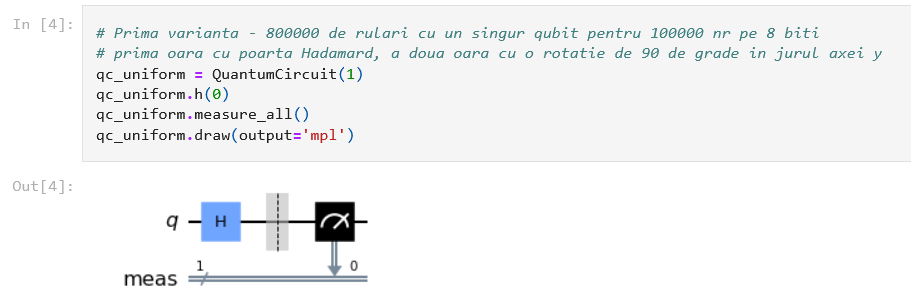
\includegraphics[width=1.0\textwidth]{anexe/figuri/CircuitHadamard1.png}
    \caption{Implementarea și figura circuitului pentru Hadamard1Bit}
    \label{fig:CircuitHadamard1BitAnexa}
\end{figure}

\begin{figure}[H]
    \centering
    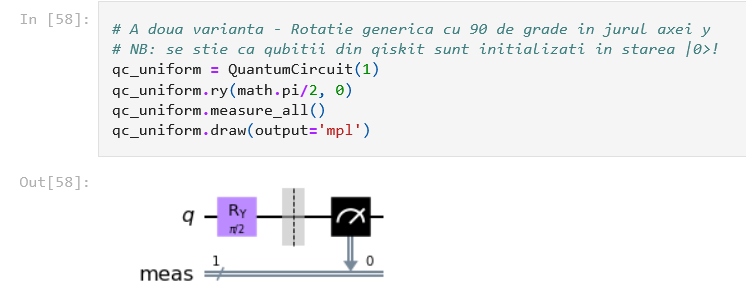
\includegraphics{anexe/figuri/CircuitRy1.png}
    \caption{Implementarea și figura circuitului pentru RY1Bit}
    \label{fig:CircuitHadamard8BitAnexa}
\end{figure}

Echivalent pentru variantele cu 8 qubiți.
Circuitele pentru normale sunt prea mari pentru a fi vizualizate.
